% Generated by scripts/2026-10-21/extract_floats.py from paper/main_en.tex; edit the full manuscript, not this file.
\begin{figure}[htbp]
\centering
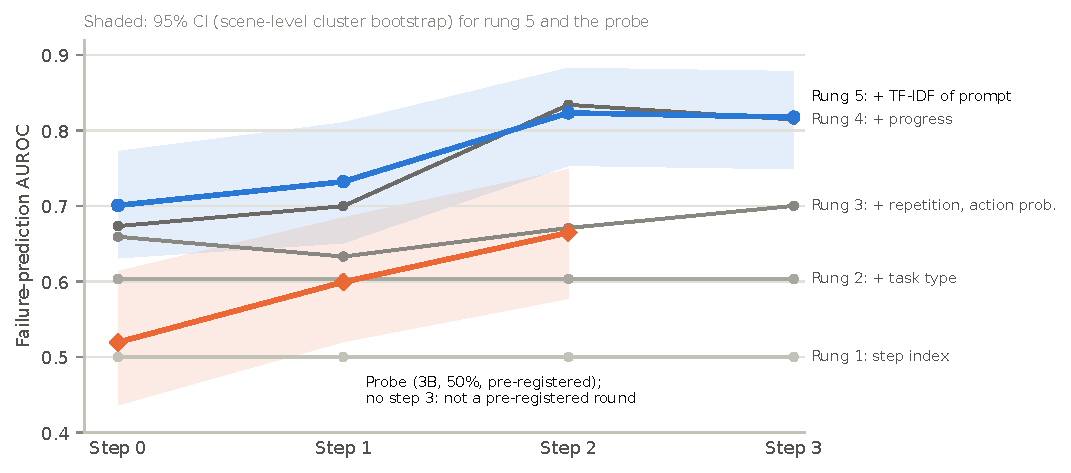
\includegraphics[width=\linewidth]{fig2_baseline_ladder.pdf}
\caption{Failure-prediction AUROC of the baseline ladder (steps 0--3) and the pre-registered probe (steps 0--2) on the first 250 episodes ($n = 250$, 194 failures per step). Rung 5 and the probe are emphasized, with shaded 95\% CIs from a scene-level cluster bootstrap (1,000 resamples); CIs of rungs 1--4 are omitted for legibility. Rung 1 is 0.5 by design and rung 2 does not change with the step. Overlap of the two shaded bands is not a test of their difference; the paired differences are in Fig.~\ref{fig:forest}.}\label{fig:ladder}
% Sources: results/baselines_main_3b.csv, results/probe_main_3b_primary.csv
\end{figure}
